\documentclass[git]{deltares_manual}

\svnid{$Id: Delft3D-MATLAB_UM.tex 79761 2024-10-16 09:47:51Z hutten $}

%------------------------------------------------------------------------------
% the following code defines a \textcode{} command that sets the text
% in verbatim mode very similar to \command{}, but it prints straight
% quotes. Unfortunately, contrary to \command{} it seems that it doesn't
% work in headings. So, this command is only used once in the compatibility
% section for a remark on rendered quotes.
%------------------------------------------------------------------------------
\ExplSyntaxOn
\NewDocumentCommand{\textcode}{v}
 {
  \ian_textcode:n { #1 }
 }

\tl_new:N \l_ian_textcode_tl

\cs_new_protected:Npn \ian_textcode:n #1
 {
  \tl_set:Nn \l_ian_textcode_tl { #1 }
  \tl_replace_all:Nnn \l_ian_textcode_tl { ' } { \textquotesingle }
  \texttt { \l_ian_textcode_tl }
 }
\ExplSyntaxOff
%------------------------------------------------------------------------------
 
% Suites
\newcommand{\dfmsuite}{Delft3D~Flexible~Mesh~Suite\xspace}
\newcommand{\dhydrosuite}{D-HYDRO~Suite\xspace}
\newcommand{\sobeksuite}{SOBEK~Suite\xspace}
\newcommand{\sobek}{SOBEK\xspace}
\newcommand{\sobekthree}{SOBEK\,3\xspace}
\newcommand{\sobektwo}{SOBEK\,2\xspace}
\newcommand{\fews}{\textrm{Delft-FEWS}\xspace}
\newcommand{\threedi}{\textrm{3Di}\xspace}
% Framework
\newcommand{\DeltaShell}{\textrm{Delta\,Shell}\xspace}
\newcommand{\deltashell}{\textrm{Delta~Shell}\xspace} % for headings where \, is not allowed
\newcommand{\dimr}{\textrm{DIMR}\xspace}
\newcommand{\dimrfull}{\textrm{Deltares Integrated Model Runner}\xspace}
% Flow modules
\newcommand{\dflowfmfull}{\textrm{D-Flow~Flexible~Mesh}\xspace}
\newcommand{\dflowfm}{\textrm{D-Flow~FM}\xspace}
\newcommand{\dflowfmonedtwod}{\textrm{D-Flow~FM~1D2D}\xspace}
\newcommand{\dflowfmtwodthreed}{\textrm{D-Flow~FM~2D3D}\xspace}
\newcommand{\dflowoned}{D-Flow\,1D\xspace}
% D-Morphology
\newcommand{\dmorphology}{\textrm{D-Morphology}\xspace}
% D-RR
\newcommand{\drainfallrunoff}{\textrm{D-Rainfall~Runoff}\xspace}
\newcommand{\drrfull}{\drainfallrunoff}
\newcommand{\drr}{D-RR\xspace}
% D-RTC
\newcommand{\drtcfull}{D-Real~Time~Control\xspace}
\newcommand{\drtc}{D-RTC\xspace}
\newcommand{\rtctools}{\textrm{RTC-Tools}\xspace}
\newcommand{\fbctools}{\textrm{FBC-Tools}\xspace}
% D-Waves
\newcommand{\dwaves}{D-Waves\xspace}
\newcommand{\swan}{SWAN\xspace}
% D-WAQ
\newcommand{\dwaqfull}{\textrm{D-Water~Quality}\xspace}
\newcommand{\dwaq}{\dwaqfull}
\newcommand{\ddido}{\textrm{D-WAQ~DIDO}\xspace}
\newcommand{\DNESTWQ}{\textrm{D-WAQ~NESTWQ}\xspace}
\newcommand{\DPART}{\textrm{D-WAQ~PART}\xspace}
\newcommand{\DPLCT}{\textrm{D-WAQ~PLCT}\xspace}
% D-SLE
\newcommand{\dslefull}{\textrm{D-SLE (Sea Lock Exchange)}\xspace}
\newcommand{\dsle}{\textrm{D-SLE}\xspace}
\newcommand{\dsledll}{\textrm{dsle.dll}\xspace}
% D-Grid Editor
\newcommand{\grideditor}{\textrm{Grid~Editor}\xspace}
\newcommand{\dgrideditor}{\textrm{D-Grid~Editor}\xspace}
% Utilities
\newcommand{\drgfgrid}{\textrm{RGFGRID}\xspace}
\newcommand{\dquickin}{\textrm{QUICKIN}\xspace}
\newcommand{\quickplot}{\textrm{QUICKPLOT}\xspace}
\newcommand{\Muppet}{Muppet\xspace}
% Open ...
\newcommand{\openmi}{OpenMI\xspace}
\newcommand{\openda}{OpenDA\xspace}
% Specific for Delft3D 4
\newcommand{\dfoursuite}{Delft3D~4~Suite\xspace}
\newcommand{\dflow}{\textrm{Delft3D-FLOW}\xspace}
\newcommand{\DWAVE}{\textrm{Delft3D-WAVE}\xspace}
\newcommand{\dmenu}{\textrm{Delft3D-MENU}\xspace}
\newcommand{\dquickplot}{\textrm{Delft3D-QUICKPLOT}\xspace}
\newcommand{\DSED}{\textrm{Delft3D-SED}\xspace}
\newcommand{\DMOR}{\textrm{Delft3D-MOR}\xspace}
\newcommand{\DTIDE}{\textrm{Delft3D-TIDE}\xspace}
\newcommand{\DTRIANA}{\textrm{Delft3D-TRIANA}\xspace}
\newcommand{\DCHEM}{\textrm{Delft3D-CHEM}\xspace}
\newcommand{\DDRIEDWAQ}{\textrm{Delft3D-WAQ}\xspace}
\newcommand{\DECO}{\textrm{Delft3D-ECO}\xspace}
\newcommand{\DGIS}{\textrm{Delft3D-GIS}\xspace}
\newcommand{\DGISVIEW}{\textrm{GISVIEW}\xspace}
\newcommand{\DGPP}{\textrm{GPP}\xspace}
\newcommand{\DMATLAB}{\textrm{Delft3D-MATLAB}\xspace}
\newcommand{\DNESTHD}{\textrm{Delft3D-NESTHD}\xspace}
\newcommand{\DOLV}{\textrm{RemoteOLV}\xspace}
\newcommand{\DREMOTEOLV}{RemoteOLV\xspace}
% Specific for SOBEK 2
\newcommand{\sobekflow}{SOBEK-FLOW\xspace}
\newcommand{\sobekonetwo}{\textrm{SOBEK-1D2D\xspace}}
\newcommand{\sbkwaq}{\textrm{SOBEK-WAQ}\xspace}
% Specific for SOBEK RE
\newcommand{\sobekrefull}{SOBEK~River Estuary\xspace}
\newcommand{\sobekre}{SOBEK-RE\xspace}
%
% For backward compatibility: capitalized keywords
%
\newcommand{\DFLOW}{\textrm{Delft3D-FLOW}\xspace}
\newcommand{\DMENU}{\textrm{Delft3D-MENU}\xspace}
\newcommand{\DQUICKPLOT}{\textrm{Delft3D-QUICKPLOT}\xspace}
\newcommand{\DRGFGRID}{\textrm{RGFGRID}\xspace}
\newcommand{\DQUICKIN}{\textrm{QUICKIN}\xspace}
\newcommand{\QUICKPLOT}{\textrm{QUICKPLOT}\xspace}
\newcommand{\DDIDO}{\textrm{D-WAQ~DIDO}\xspace}
\newcommand{\DFLOWFMfull}{\dflowfmfull}
\newcommand{\DFLOWFM}{\dflowfm}
\newcommand{\DRRfull}{\drainfallrunoff}
\newcommand{\DRR}{\drr}
\newcommand{\DRTCfull}{\drtcfull}
\newcommand{\DRTC}{\drtc}
\newcommand{\RTCTOOLS}{\rtctools}
\newcommand{\FBCTOOLS}{\fbctools}
\newcommand{\SWAN}{\swan}
\newcommand{\DWAQfull}{\dwaqfull}
\newcommand{\DWAQ}{\dwaq}
\newcommand{\OPENMI}{\openmi}
\newcommand{\OPENDA}{\openda}

% GUI names 
\newcommand{\maptree}{Map~Tree\xspace}
\newcommand{\projectwindow}{Project~Window\xspace}
\newcommand{\projecttree}{Project~Tree\xspace}
\newcommand{\gridnodes}{Grid~Nodes\xspace}

\newcommand{\maptab}{Map~tab\xspace}
\newcommand{\gridtab}{Grid~tab\xspace}
\newcommand{\hometab}{Home~tab\xspace}
\newcommand{\spatialtab}{Spatial~Operations~tab\xspace}


\newcommand{\vsuse}{\command{vs\_use}}
\newcommand{\vsdisp}{\command{vs\_disp}}
\newcommand{\vslet}{\command{vs\_let}}
\newcommand{\vsget}{\command{vs\_get}}
\newcommand{\vstype}{\command{vs\_type}}
\newcommand{\vsfind}{\command{vs\_find}}
\newcommand{\vsdiff}{\command{vs\_diff}}

%------------------------------------------------------------------------------
\makeatletter
\version{2.72}
\hypersetup
{
    pdfauthor   = {Deltares},
    pdftitle    = {\DMATLAB\ User Manual},
    pdfkeywords = {Deltares User Manual MATLAB \DMATLAB}
}
\makeatother

%------------------------------------------------------------------------------
%
\renewcommand\BackgroundPicChapter{
    \put(0,0){
    \parbox[b][\paperheight]{\paperwidth}{%
        \vspace{4\baselineskip}
        \hspace{220mm}
        
\includegraphics[width=15mm]{pictures/delft3d-chapter-ribbon.jpg}%
        \vfill
        }
    }
}

%------------------------------------------------------------------------------
%
\begin{document}
\pagestyle{empty}
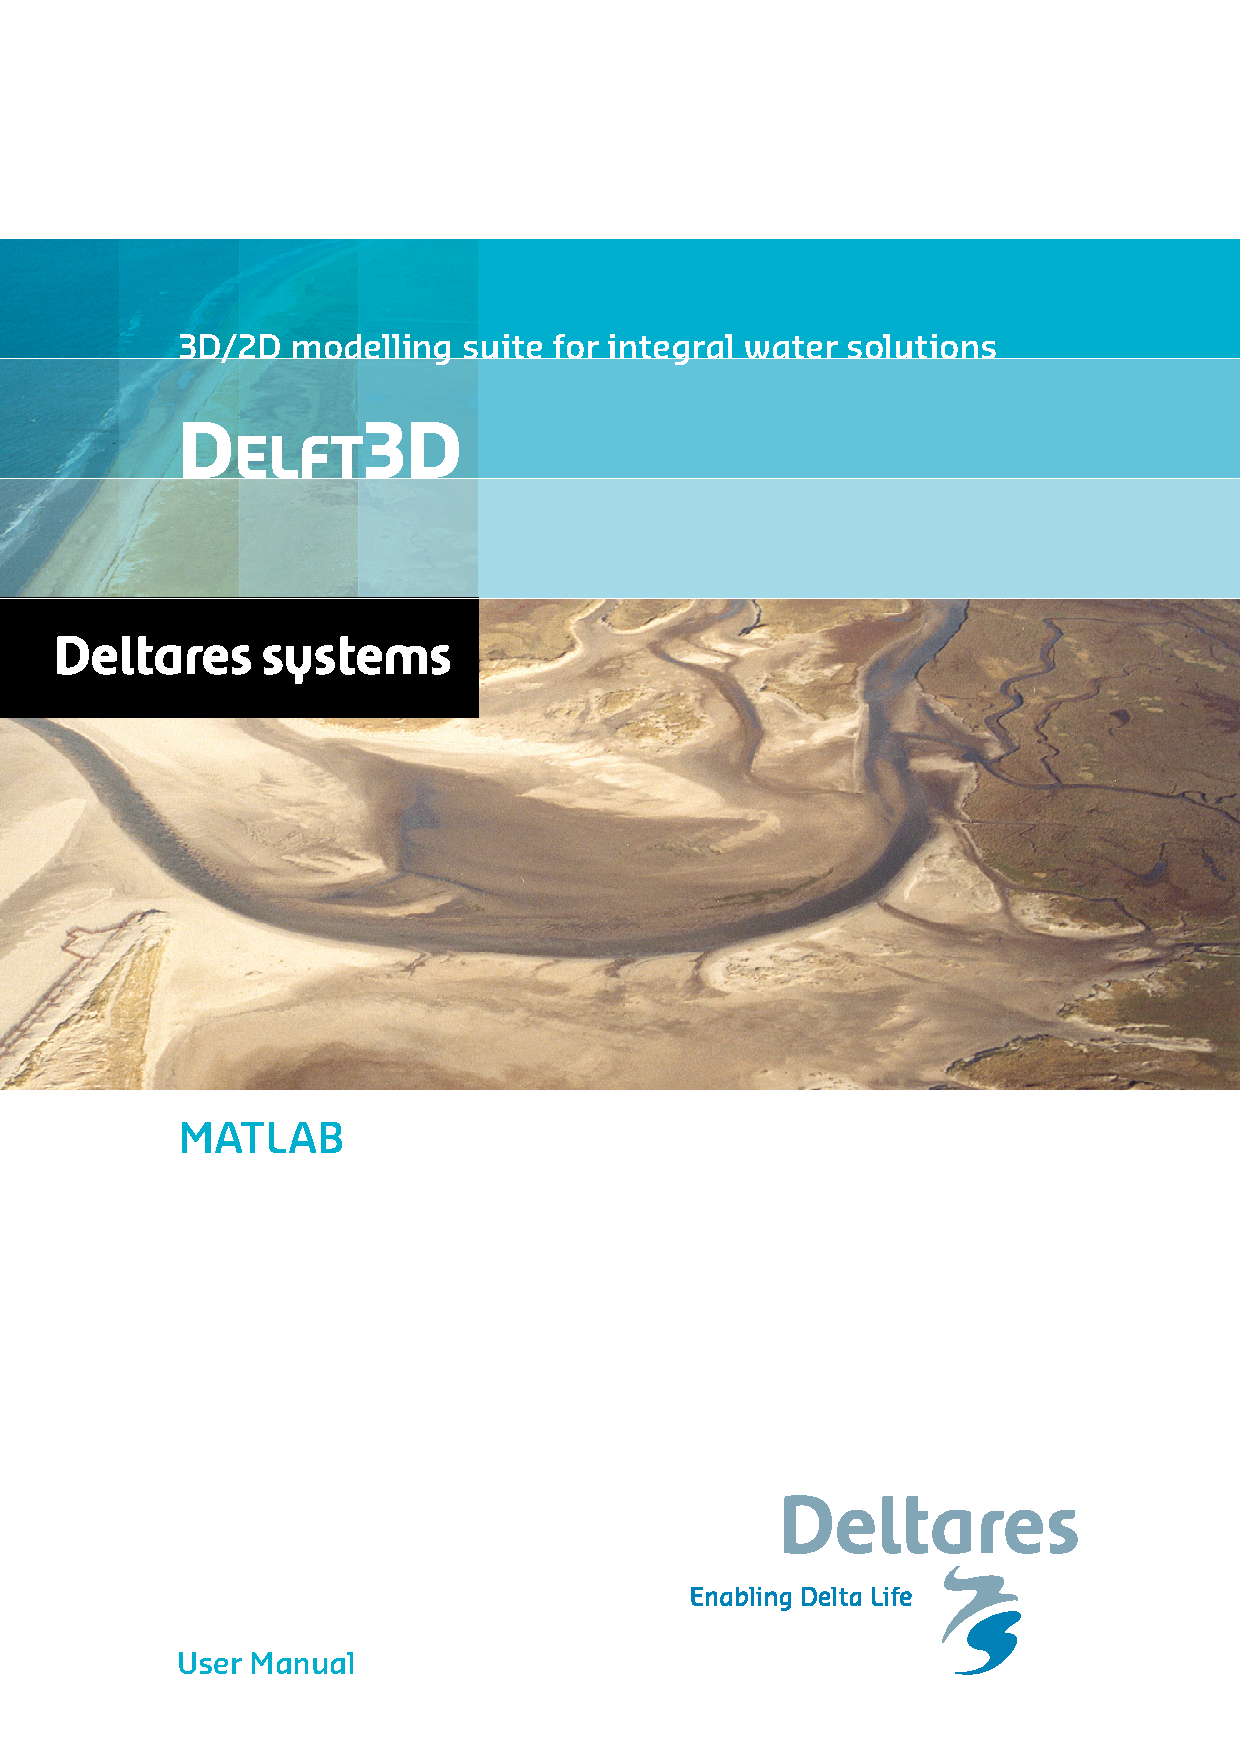
\includepdf[pages=1,offset=72 -70]{pictures/delft3d-cover_matlab.pdf} % links-rechts past precies
\cleardoublepage

\title{\DMATLAB}
\subtitle{Interface to MATLAB for flexibility in visualisation and data analysis}
\manualtype{User Manual}
\distribution{Hydro-Morphodynamics \& Water Quality}
\manualtitle

\svnid{$Id: introduction.tex 74563 2022-02-13 20:35:17Z jagers $}

\chapter{Introduction}
The MATLAB interface for Delft3D has been developed to expand the flexibility in the processing of Delft3D data in general and of NEFIS data files in particular.
The interface consists of three parts:

\begin{itemize}
\item First, generic low level routines to access data stored in NEFIS files by the \dfoursuite.
The routines are described in the second chapter of this manual.
A thorough knowledge of the Delft3D system is required.

\item Second, high level routines to access the data.
This includes routines for reading and writing \dflow restart files, grid and depth files.
Routines to load and plot grid, thin dams, and velocity data directly from the \dfoursuite result files.
Finally a set of routines to open and read data from any file supported by QUICKPLOT; this includes the result files of both the \dfoursuite and the \dfmsuite.
For a full overview of all supported file formats see the appendix of \citet{QP_UM}.
These routines are described in Chapter \ref{Chp:HighLevelRoutines}.

\item Third, a graphical user interface for basic plotting.
The QUICKPLOT\ interface is described in Chapter \ref{Chp:QuickPlot}.
\end{itemize}

All functions are provided in source code under LGPL v2.1 conditions.
The routines described in chapters three and four can be used as examples for development of other routines.

\section{Version information}
This manual describes the functionality of \DMATLAB\ interface version 2.60 and later versions.

\section{Compatibility}
The routines have been tested for compatibility with MATLAB versions ranging from 6.5 (R13) until 2022a.
Although quotes in commands are sometimes rendered in this manual as \command{'}, every quote is intended to be a straight quote \textcode{'}.


\svnid{$Id: lowlevel.tex 74563 2022-02-13 20:35:17Z jagers $}

\chapter{Low level routines} \label{Chp:LowLevelRoutines}
A set of MATLAB files has been created to access NEFIS files from within MATLAB.
The following functions have been implemented:

\begin{guilist}
\item[\vsuse] open NEFIS file
\item[\vsdisp]display information of groups and elements contained in a NEFIS file
\item[\vslet/\vsget] get data from a NEFIS file
\item[\vstype] determine type of a NEFIS file
\item[\vsfind] find group to which an element belongs
\item[\vsdiff] find differences between two NEFIS files
\end{guilist}

If no NEFIS file is specified when using the commands \vsdisp, \vslet, \vsget, \vstype~and \vsfind~the last opened NEFIS is used.
The commands are discussed below in more detail.

\begin{Remark}
\item Spatial data sets are stored in the NEFIS file with the M and N dimensions reversed.
\end{Remark}

\section{Open NEFIS file: \vsuse}

\subsection*{Purpose}
Open/scan NEFIS file

\subsection*{Syntax}
\begin{Verbatim}
Nfs = vs_use(FileName)
\end{Verbatim}

\subsection*{Description}
\command{Nfs = vs\_use(FileName)} opens a NEFIS file where the filename is the name of either the definition or the data file, and returns a handle \command{Nfs} to the file, which must be used when calling the other commands.
When no filename is specified, the command will ask for one.

The \vsuse command scans the structure of the definition and data files; this will take some time.
MATLAB can store the structure information in a file with the same name base (as indicated by filename) and extension \file{$\ast$.mat}, and read that information when the file is re-opened a next time.
This used to be the default behaviour but is now optional: use option usemat.
The old option nomat is still accepted and overrules usemat.
If changes were made to the \file{$\ast$.def} and/or \file{$\ast$.dat} files, you should add refresh as additional argument to prevent reading the existing mat-file.
The addition of the argument quiet as last argument reads the file structure without showing the wait bar.
When the option debug is used a file \file{vs\_use.dbg} is created in the default temporary directory, containing information on the reading of the data structure from the NEFIS file.

The returned \command{Nfs} can be interpreted as a file handle as used in all programming environments for file access.
However, it is not an integer but a structure containing the internal structure of the NEFIS file.

\subsection*{Example}
\begin{Verbatim}
>> Nfs=vs_use

Nfs =

    FileName: `I:\OCTOPUS\sbod_gf3.66_tot\output\TS11520000\com-d16'
      DatExt: `.dat'
      DefExt: `.def'
      Format: `b'
      gNames: [21x368 char  ]
       gData: [21x27  double]
      eNames: [89x112 char  ]
       eData: [89x11  double]
\end{Verbatim}

\section{Display information of groups and elements: \vsdisp}

\subsection*{Purpose}
Display NEFIS file contents.

\subsection*{Syntax}
\begin{Verbatim}
vs_disp(Nfs)
Output = vs_disp(Nfs)
vs_disp(Nfs, [])
Output = vs_disp(Nfs, [])
vs_disp(Nfs, GroupName)
Output = vs_disp(Nfs, GroupName)
Output = vs_disp(Nfs, GroupName, [])
Output = vs_disp(Nfs, GroupName, ElementName)
\end{Verbatim}

\subsection*{Description}
\command{vs\_disp(Nfs)} lists all group names, group elements, and all group and element properties like the \command{disp stat} command of the Viewer Selector.
\command{vs\_disp(Nfs, [])} lists group names, group dimensions, and number of elements per group only.
This can be used as a short summary of the file contents.
\command{Output = vs\_disp(Nfs)} and \command{Output = vs\_disp(Nfs, [])} return a char matrix containing the names of the groups.

\command{vs\_disp(Nfs, GroupName)} lists all group elements, and all element properties like the \command{disp GroupName} command of Viewer Selector.
\command{Output = vs\_disp(Nfs, GroupName)} returns a char matrix containing the names of the elements of the group.

\command{Output = vs\_disp(Nfs, GroupName, [])} gives detailed data about the specified group contained in the Nfs structure.
The information includes group data name, cell name, definition name, number of elements, dimensions, and the offsets within the NEFIS file at which locations data of the group are stored.
\command{Output = vs\_disp(Nfs, GroupName, ElementName)} gives detailed data about the specified element contained in the Nfs structure.
The information includes element description, unit and size.

\subsection*{Examples}
\begin{Verbatim}
>> vs_disp(Nfs)
Groupname:BOTNT            Dimensions:(1)
  No attributes
    NTBOT          INTEGER *  4             [   -   ]       ( 1 )
        Number of bottom fields in group BOTTIM

Groupname:BOTTIM           Dimensions:(24)
  No attributes
    TIMBOT         INTEGER *  4             [ TSCALE]       ( 1 )
        Communication times bottom fields rel. to reference date/time
    DP             REAL    *  4             [   M   ]      ( 98 62 )
        Bottom depth in bottom points, positive downwards
\end{Verbatim}
and so on ...
\begin{Verbatim}


>> vs_disp(Nfs,[])
BOTNT           (1) - No attributes, 1 element(s).
BOTTIM          (24)  No attributes, 2 element(s).
PARAMS          (1) - No attributes, 8 element(s).
GRID            (1) - No attributes, 16 element(s).
SPECPOINTS      (1) - No attributes, 4 element(s).
BOUNDCNST       (1) - No attributes, 8 element(s).
KENMCNST        (1) - No attributes, 3 element(s).
INITBOT         (1) - No attributes, 4 element(s).
ROUGHNESS       (1) - No attributes, 3 element(s).
TEMPOUT         (1) - No attributes, 4 element(s).
com-version     (1) - No attributes, 3 element(s).
KENMNT          (1) - No attributes, 1 element(s).
KENMTIM         (1) - No attributes, 3 element(s).
CURNT           (1) - No attributes, 1 element(s).
CURTIM          (1) - No attributes, 7 element(s).
DWQTIM          (1) - No attributes, 5 element(s).
TAUTIM          (1) - No attributes, 1 element(s).
INITI           (1) - No attributes, 1 element(s).
TRANNT          (1) - No attributes, 2 element(s).
BOUNDMOR        (1) - No attributes, 1 element(s).
TRANSTIM        (1) - No attributes, 11 element(s).


>> Output=vs_disp(Nfs) %or Output=vs_disp(Nfs,[])

Output =

BOTNT
BOTTIM
PARAMS
GRID
SPECPOINTS
BOUNDCNST
KENMCNST
INITBOT
ROUGHNESS
TEMPOUT
com-version
KENMNT
KENMTIM
CURNT
CURTIM
DWQTIM
TAUTIM
INITI
TRANNT
BOUNDMOR
TRANSTIM


>> vs_disp(Nfs,`BOTTIM')
Groupname:BOTTIM           Dimensions:(24)
  No attributes
    TIMBOT         INTEGER *  4            [ TSCALE]        ( 1 )
        Communication times bottom fields rel. to reference date/time
    DP             REAL    *  4            [   M   ]       ( 98 62 )
        Bottom depth in bottom points, positive downwards


>> Output=vs_disp(Nfs,`BOTTIM')

Output =

TIMBOT
DP


>> Output=vs_disp(Nfs,`BOTTIM',[]) % get group information

Output =

              Name: `BOTTIM'
    GroupDatOffset: 8560
           DefName: `BOTTIM'
    GroupDefOffset: 12728
          CellName: `BOTTIM'
     CellDefOffset: 12660
         CellNByte: 24308
          CellNElm: 2
              NDim: 1
            VarDim: 1
           SizeDim: 24
          OrderDim: 1
            Attrib: [1x1 struct]


>> Output=vs_disp(Nfs,`BOTTIM',`DP') % get element information

Output =

          GrpNname: `BOTTIM'
           ElmName: `DP'
       ElmQuantity: `'
          ElmUnits: `[   M   ]'
    ElmDescription: `Bottom depth in bottom points, positive downwards'
      ElmDefOffset: 12496
              NDim: 2
           SizeDim: [98 62]
           TypeVal: 5
          NByteVal: 4
             NByte: 24304
\end{Verbatim}

\section{Get data from a NEFIS file: \vslet/\vsget}

\subsection*{Purpose}
 Read data from file (groups as columns or cells).

\subsection*{Syntax}
\begin{Verbatim}
[Data, Succes] = vs_let(Nfs, GroupName, GroupIndex, ElementName, ElementIndex)
[Data, Succes] = vs_get(Nfs, GroupName, GroupIndex, ElementName, ElementIndex)
\end{Verbatim}

\subsection*{Description}
\begin{Verbatim}
Data = vs_let(Nfs, GroupName, GroupIndex, ElementName, ElementIndex)
Data = vs_get(Nfs, GroupName, GroupIndex, ElementName, ElementIndex)
\end{Verbatim}

These commands read the requested element from the specified group from the specified file.
The \command{GroupIndex} should be a 1xN cell array, where N equals the number of dimensions of the group.
Each element of the cell array should contain either 0 (zero) or the indices of the cells that should be read.
The 0 means that all cells should be read.
The \command{ElementIndex} should be a 1xM cell array, where M equals the number of dimensions of the element.
Again, each element of the cell array should contain either 0 (zero) or the indices of the elements that should be read, where 0 means that the complete dimension should be read.
When the option debug is used a file \file{vs\_let.dbg} is created in the default temporary directory, containing information on the reading of the data from the NEFIS file.

The command \vslet~reads all data in one big matrix, using the first dimensions for the groups and the last dimensions for the elements.
The command \vsget~returns a matrix containing the data if data from only one group is read, and a cell array of matrices when data from more than one group is read.
An additional output option succes \command{[Data,Succes] = ...} indicates whether the data has been read successfully.

When the \command{GroupIndex} and/or \command{ElementIndex} are skipped all fields of the group/element are selected.
When no \command{GroupName} or \command{ElementName} is specified or when an error is encountered while interpreting the input a graphical user interface is presented to enter the selection.
To help new users to get acquainted to the command line syntax of the \vsget~and \vslet~routines, the command option line \command{-cmdhelp} is provided.
When used, the routine does not actually load the data, but it displays the command line equivalent of the selection that you have made in the user interface.

\subsection*{Examples}
 For example: To read from the depth data the first 10 rows (and of those rows all columns) of the 1st, 3rd, 5th, 7th, and 9th time steps, you should type:

\begin{Verbatim}
>> Data=vs_let(Nfs,`BOTTIM',{1:2:10},`DP',{1:10 0});
\end{Verbatim}

which returns a 5x10x62 matrix; or

\begin{Verbatim}
>> Data=vs_get(Nfs,`BOTTIM',{1:2:10},`DP',{1:10 0})

Data =

    [10x62 double]
    [10x62 double]
    [10x62 double]
    [10x62 double]
    [10x62 double]
\end{Verbatim}

Indicating that a 5 x 1 cell array is returned, each cell containing one bottom field (10 x 62 data points).
Character strings are contained in cell arrays.
The most common cases of reading from are:

\begin{Verbatim}
Data=vs_get(Nfs,`BOTTIM',{0},`DP',{0 0})
\end{Verbatim}

Read all bottom data completely.
Group/Element indices containing only zeros don't have to be specified.
So, the following is also accepted:

\begin{Verbatim}
Data=vs_get(Nfs,`BOTTIM',`DP')

Data=vs_get(Nfs,`BOTTIM',{0},`DP',{n 0}), or
Data=vs_get(Nfs,`BOTTIM',`DP',{n 0})
\end{Verbatim}

Read cross-section n at all time steps

\begin{Verbatim}
Data=vs_get(Nfs,`BOTTIM',{t},`DP',{0 0}), or
Data=vs_get(Nfs,`BOTTIM',{t},`DP')
\end{Verbatim}

Read the bottom at time step t.
This will return a 10 x 62 matrix if \vsget~is used, and a 1x10x62 matrix if \vslet~is used.

\begin{Verbatim}
Data=vs_get(Nfs,`BOTTIM',{0},`DP',{n m}), or
Data=vs_get(Nfs,`BOTTIM',`DP',{n m})
\end{Verbatim}

Read the variation of the bottom at indicated (n,m)-point.
If this is followed by a \command{Data = [Data{:}];} command to convert the cell array containing single values into a vector; it can be replaced by

\begin{Verbatim}
Data=vs_let(Nfs,`BOTTIM',`DP',{m n})
\end{Verbatim}

which gives that result immediately and is faster.

When besides the \command{Nfs} no further arguments are used (or when no element name is specified), an interface will appear asking for the other arguments.
Adding the string \command{quiet} as last input argument will suppress the wait bar during loading.
When \command{`*'} is specified as element name all elements of the group are returned; if an element index is specified it is ignored.

\subsection*{Example}
\begin{Verbatim}
Data=vs_let(Nfs,`BOTTIM',{1:2:10},`*')
\end{Verbatim}

returns

\begin{Verbatim}
Data =

   TIMBOT: [5x1     double]
       DP: [5x10x62 double]
\end{Verbatim}

and

\begin{Verbatim}
Data=vs_get(Nfs,`BOTTIM',{1:2:10},`*')
\end{Verbatim}

returns the data of five time steps

\begin{Verbatim}
Data =

5x1 struct array with fields:
    TIMBOT
    DP
\end{Verbatim}

To assist the novice user with the syntax of the \vslet~and \vsget~commands a help functionality has been added to these functions which allows the interactive generation of command lines.
This functionality is activated by supplying \command{-cmdhelp} as one of the input arguments.
For instance:

\begin{Verbatim}
>> vs_let -cmdhelp
\end{Verbatim}

results after the following data has been entered in the user interface in the following output string

\begin{Verbatim}
Data=vs_let(NFStruct,`BOTTIM',{[ 1:2:9 ]},`DP',{[ 1:10 ],0});
\end{Verbatim}

You can copy this string into a text editor for use in a script.
As indicated above, variations on the syntax are allowed.
The following line is also valid

\begin{Verbatim}
Data=vs_let(`BOTTIM',{1:2:9},`DP',{1:10,1:73});
\end{Verbatim}

The result will be exactly the same provided that the variable NFStruct in the first command line contains the information of the last opened NEFIS file.

\section{Determine the type of a NEFIS file: \vstype}

\subsection*{Purpose}
Show type of NEFIS file.

\subsection*{Syntax}
\begin{Verbatim}
Type=vs_type(Nfs)
\end{Verbatim}

\subsection*{Description}
The function returns the type of the loaded NEFIS file.
Currently the following NEFIS files are detected: `Delft3D-com', `Delft3D-trim', `Delft3D-trih', `Delft3D-trid', `Delft3D-tram', `Delft3D-trah', `Delft3D-botm'.
Other NEFIS files will return `unknown'.
For example:

\subsection*{Example}
\begin{Verbatim}
>> Type=vs_type(Nfs)

Type =

Delft3D-com
\end{Verbatim}

\section{Find group to which element belongs: \vsfind}

\subsection*{Purpose}
Find elements in a NEFIS file.

\subsection*{Syntax}
\begin{Verbatim}
Groups=vs_find(Nfs, ElementName)
\end{Verbatim}

\subsection*{Description}
The function returns a list of group names containing the specified element.
For example the element `TIMCUR' occurs in several groups of the com-file:

\subsection*{Example}
\begin{Verbatim}
>> Groups=vs_find(Nfs,`TIMCUR')

Groups =

KENMTIM
CURTIM
DWQTIM
\end{Verbatim}

\section{Find differences between two NEFIS files: \vsdiff}

\subsection*{Purpose}
Compare NEFIS file contents and find differences in groups, elements and data.

\subsection*{Syntax}
\begin{Verbatim}
vs_diff(Nfs1,Nfs2)
\end{Verbatim}

\subsection*{Description}
The function analyses the specified NEFIS files for differences.
The analyses searches first for differences in the contained groups.
If it finds differences it stops, if not it continues to search for differences in the elements, element properties, and element data.

\subsection*{Example}
The following comparison between two com-files, of which the first was obtained by a restart run from the second one, indicates

\begin{itemize}
\item differences in the water and sediment transport data fields;
\item a difference in the group properties of the BOTTIM group (which is caused by one additional depth field); and
\item differences in the `RUNTXT' and `SIMDAT' texts.
\end{itemize}

\begin{Verbatim}
>> vs_diff(Nfs,Nfs2)
Comparing NEFIS files ...
File 1: I:\OCTOPUS\sbod_gf3.66_tot\output\TS11520000\com-d16
File 2: I:\OCTOPUS\sbod_gf3.66_tot\output\TS11160000\com-d16

Data of element NTBOT of group BOTNT differ.
Group properties differ for: BOTTIM
Data of element QU of group CURTIM differ.
Data of element QV of group CURTIM differ.
Data of element S1 of group CURTIM differ.
Data of element TIMCUR of group CURTIM differ.
Data of element U1 of group CURTIM differ.
Data of element V1 of group CURTIM differ.
Data of element TIMCUR of group DWQTIM differ.
Data of element KFU of group KENMTIM differ.
Data of element KFV of group KENMTIM differ.
Data of element TIMCUR of group KENMTIM differ.
Data of element TAUMAX of group TAUTIM differ.
Data of element TSEDB of group TRANSTIM differ.
Data of element TSEDE of group TRANSTIM differ.
Data of element TTXA of group TRANSTIM differ.
Data of element TTYA of group TRANSTIM differ.
Data of element RUNTXT of group com-version differ.
Data of element SIMDAT of group com-version differ.
... comparison finished.
\end{Verbatim}

\svnid{$Id: highlevel.tex 74563 2022-02-13 20:35:17Z jagers $}

\chapter{High level routines} \label{Chp:HighLevelRoutines}
Although the low level routines provide access to all data in the NEFIS files, obtaining a useful, consistent data set can be difficult.
For instance, to plot a 2D vector field you have to combine the information stored at about seven locations in the Delft3D communication file.
Therefore, a number of high level routines has been provided to simplify the plotting and data retrieval operations.
Routines are provided for plotting a grid (with grid number labels), plotting thin dams and inactive velocity points, and retrieving data to plot velocity vectors.
Functions are also provided for reading and writing \DRGFGRID\  grid files (\DRGFGRID\  manual~\citep{RGF_UM}), \DQUICKIN\ depth files (\DQUICKIN\ manual~\citep{QUICKIN_UM}, and \DFLOW\ restart files (\DFLOW\ manual~\citep{FLOW_UM}).

\section{Plot a grid: \command{drawgrid}}

\subsection*{Purpose}
Plot the morphological grid.

\subsection*{Syntax}
\begin{Verbatim}
drawgrid(NFStruct)
[X, Y] = drawgrid(NFStruct);
drawgrid(X, Y)
\end{Verbatim}

\subsection*{Description}
\command{drawgrid(NFStruct)} where \command{NFStruct} is the structure obtained from the \vsuse\ command.
The function adds the morphological grid (that is, the user-defined grid) to the current axes.
\file{trim-$\ast$}, \file{tram-$\ast$}, \file{botm-$\ast$}, and \file{com-$\ast$} files are supported.
The morphological grid equals the grid specified in the input file; the bed level points are specified on the grid line crossings.

\command{[X, Y] = drawgrid(NFStruct)} returns the X and Y co-ordinates, but it does not actually draw the morphological grid.

\command{drawgrid(X, Y)} draws the user specified grid in the current axes.

This function accepts a number of optional arguments, which consist of property - value pairs similar to those use by the MATLAB \command{set} command:
\command{drawgrid(..., 'optionname1', optionval1, 'optionname2', optionval2, ...)}.
The supported options are

\begin{guilist}
\item['color'] The value can be an RGB-triplet, a colour character ('r', 'g', 'b', 'c', 'm', 'y', 'k', 'w'), or the string 'ortho' for colouring based on the orthogonality of grid, 'msmo' for the M-smoothness of grid, 'nsmo' for the N-smoothness of grid
\item['m1n1'] $[N M]$ number of grid point(1,1).
Useful when plotting only part of the grid.
\item['fontsize'] The size of the font used for grid numbering (default 4)
\item['gridstep'] Label step used for grid numbering (default 10).
For instance, 5 will number every fifth grid line.
If grid step is [], grid lines are not labelled.
\item['thicklength'] Length of ticks in axes co-ordinates or 'auto' (default)
\item['parent'] The axes handle in which to plot grid (default the current axes, gca)
\item['clipzero'] By default co-ordinate pairs of (0,0) are clipped.
Set to 'off' to plot co-ordinates at (0,0))
\end{guilist}

\subsection*{Example, \Fref{fig:3-1}}
\begin{Verbatim}
>> G=wlgrid('read','d:\f-disk\users\mooiman\delft3d\models\f34\f34\f34.grd')

G =

                   X: [14x21 double]
                   Y: [14x21 double]
           Enclosure: [19x2 double]
            FileName: 'D:\delft3d\tutorial\flow\f34_demo\fti_02.grd'
    CoordinateSystem: 'Cartesian'
        MissingValue: 0
                Type: 'RGF'


>> drawgrid(G.X,G.Y,'fontsize',8,'gridstep',4)
>> set(gca,'dataaspectratio',[1 1 1])
\end{Verbatim}

\begin{figure}
\center{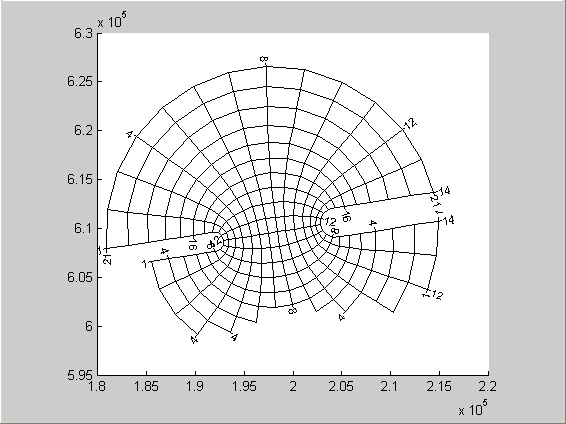
\includegraphics[width=100mm]{matlab/3-1.png}}
\caption{Grid layout from the Friesian Tidal Inlet model.}
\label{fig:3-1}
\end{figure}

\section{Plot thin dams: \command{thindam}}

\subsection*{Purpose}
Plot dams, weirs and vanes.

\subsection*{Syntax}
\begin{Verbatim}
thindam(NFStruct, T)
thindam(NFStruct, T, '3D')
thindam(XCOR, YCOR, UDAM, VDAM)
thindam('xyw', XDAM, YDAM, WDAM)
thindam(..., 'PropertyName', PropertyValue)
H = thindam(...)
[X, Y] = thindam(...)
[X, Y, M, N] = thindam(...)
[X, Y, Z] = thindam(...)
[X, Y, BOTTOM, TOP] = thindam(...)
[X, Y, BOTTOM, TOP, M, N] = thindam(...)
\end{Verbatim}

\subsection*{Description}
\command{thindam(NFStruct,T)} plots the KFU/V (drying/flooding) dams for time step T if T>0.
It plots the KCU/V thin dams if T==0 (default if T is not specified).
The function supports \file{trim-*} and \file{com-*} files.

\command{thindam(NFStruct, T, '3D')} same as above but now the dams will be plotted as 3D surfaces based on the bottom and water level information in the specified NEFIS file, \file{trim-*} or \file{com-*} file.

\command{thindam(XCOR, YCOR, UDAM, VDAM)} plots the specified U and V dams on the specified grid.
The XCOR and YCOR represent the bottom points.
Valid entries for UDAM and VDAM are:
\begin{itemize}
\item matrix of same size as XCOR/YCOR with a 1 representing a dam and a 0 indicating no dam.
\item D x 2 matrix specifying the N, M co-ordinates of the dams
\item D x 4 matrix specifying the begin/end N, M co-ordinates of the dams like in the Delft3D input files.
\end{itemize}

\command{thindam('xyw', XDAM, YDAM, WDAM, ...)} plots dams with their centre at specified (XDAM, YDAM) locations with specified width/length WDAM.
This function is useful for non-grid oriented dams.

A 3D effect can be added to these user-specified dams by specifying bottom and top levels using \command{thindam(..., 'bottom', <bottom\_args>, 'top', <top\_args>)}.
It plots the dams as 3D surfaces with specified top and bottom elevations.
The elevation data should be specified with positive direction up.
Additional supported options are:

\begin{itemize}
\item \command{'angle', <angle\_args>}
The dams/vanes are rotated to match the specified angle in degrees with respect to the positive X-axis  (positive angle in anti-clockwise direction).
\item \command{'color', <color\_args>}
The dams are coloured using the specified data.
\item \command{'thickness', <thickness\_args>}
The thickness of the dams is specified (default 0).
\end{itemize}

Valid entries for all options are:
\begin{itemize}
\item a constant, uniform value for all dams
\item a matrix of same size as XCOR/YCOR containing data in the depth points.
\item a matrix of same size as XCOR/YCOR containing data in the water level points.
To distinguish this entry from the former you need to add the string 'H' or 'S' as an extra argument after the matrix.
For example \command{thindam(..., 'top', ELEVMATRIX, 'H', ...)} indicates that the top level of the dams are derived from the specified data in water level points (the value will be used uniformly along each elementary dam).
\item two matrices of same size as XCOR/YCOR containing data in the U and V points.
\item two D x s arrays specifying the property of the individual dams.
If the array is D x 1 the value is constant along each elementary dam.
If the array is D x 2 the first value is taken for the dam end with lowest (N,M) while the second elevation for the dam end with highest (N,M).
The first array specifies the elevation for dams in U direction the second array for dams in the V direction.
For example \command{thindam(..., 'top', ELEVU, ELEVV, ...)}.
This option cannot be used in combination with option 1 for the UDAM and VDAM entries.
The number of values should match the number of dam records/elementary dams.
\end{itemize}

If a colour data field has been specified, there are a few more options available:

\begin{itemize}
\item \command{'shape',<type>} \\
The dam shape: 'dam' (default) or 'rhombus'.
\item \command{'drawdams',<onoff>}\\
Flag to draw dams.
Can be set to 'on' (default) or 'off'.
\item \command{'drawlabels',<onoff>}\\
Flag to draw the colour values as text labels.
Can be set to 'on' or 'off' (default).
\item \command{'labelformat',<format>}\\
Defines the format for displaying the values (default '\%g')
\item \command{'fontsize',<size>}\\
Defines the size of the labels.
\end{itemize}

If the 'xyw' syntax is used, then valid entries for the options are
\begin{itemize}
\item a constant (uniform value for all dams), and
\item a matrix of same size as XDAM/YDAM/WDAM.
\end{itemize}

\command{H = thindam(...)} returns the handle of the line/surface object used for plotting the dams.

\command{[X, Y] = thindam(...)} returns the x,y-arrays normally used for plotting.
The dams are not plotted.
This syntax is only valid if the input arguments indicate a 2D dam plot.

\command{[X, Y, M, N] = thindam(...)} returns four nx2 matrices containing per row a pair of end points for an elementary dam (X and Y co-ordinates, M and N index).
This syntax is only valid if the input arguments indicate a 2D dam plot.

\command{[X, Y, Z] = thindam(...)} returns the x,y,z-arrays normally used for plotting.
The dams are not plotted.
This syntax is only valid if the input arguments indicate a 3D dam plot.

\command{[X, Y, BOTTOM, TOP] = thindam(...)} returns four nx2 matrices containing per row a pair of end points for an elementary dam: X co-ordinates, Y co-ordinates, bottom elevation and top elevation.
This syntax is only valid if the input arguments indicate a 3D dam plot.

\command{[X, Y, BOTTOM, TOP, M, N] = thindam(...)} returns six nx2 matrices containing per row a pair of end points for an elementary dam: X co-ordinates, Y co-ordinates, bottom elevation, top elevation, M index, N index.
This syntax is only valid if the input arguments indicate a 3D dam plot.

\subsection*{Example, \Fref{fig:3-2}}
\begin{Verbatim}
>> vs_use D:\wl\delft3d\tutorial\wave\Siu-Lam\Com-siu
>> drawgrid('color','g')
>> set(gca,'DataAspectRatio',[1 1 1])
>> thindam(1)
>> l=thindam; set(l,'color','r')
\end{Verbatim}

\begin{figure}
\center{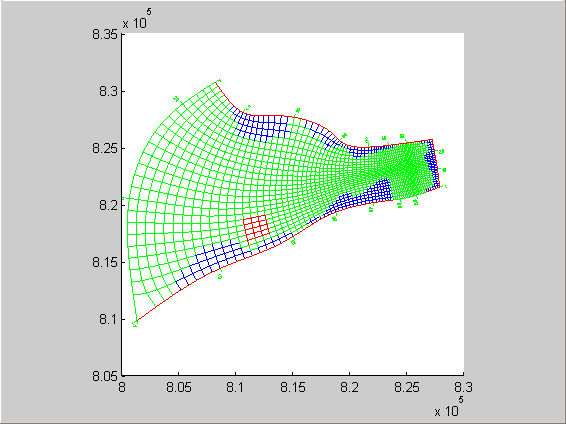
\includegraphics[width=100mm]{matlab/3-2.png}}
\caption{Example of grid and thin dams.}
\label{fig:3-2}
\end{figure}

\section{Read/write restart file: \command{trirst}}

\subsection*{Purpose}
Read/write \DFLOW\ restart file.

\subsection*{Syntax}
\begin{Verbatim}
[H, U, V, ...] = trirst('read', FILENAME, SIZE)
[H, U, V, ...] = trirst('read', FILENAME, GRID)
[H, U, V, ...] = trirst('read', FILENAME, GRID, NLAYERS)
trirst('write', FILENAME, H, U, V, ...)
trirst('write', FILENAME, PLATFORM, H, U, V, ...)
\end{Verbatim}

\subsection*{Description}
\command{[H, U, V, ...] = trirst('read', FILENAME, SIZE)} and
\command{[H, U, V, ...] = trirst('read', FILENAME, GRID)} where GRID was read in from the \file{$\ast$.grd} file by WLGRID read data from a \DFLOW\ restart file of a 2D simulation.
The dimensions of the underlying grid must be specified.
This can be done either by manually specifying the grid size as [M N], or by automatic derivation from a grid.

\command{[H, U, V, ...] = trirst('read', FILENAME, GRID, NLAYERS)} reads data from a \DFLOW\ restart file of a 3D simulation.
The NLAYERS arrays indicate the number of layers used for the various variables.
In the example syntax: \command{NLAYERS = [NLAYERH, NLAYERU, NLAYERV, ...]}.

\command{trirst('write', FILENAME, H, U, V, ...)} writes the specified matrices to the indicated restart file.
Because the restart file is stored in a platform dependent manner, care should be taken to write the appropriate type of restart file.
By default the routine writes the data in the format compatible with the computer on which MATLAB is running.
A different platform can be chosen by using the following syntax:
\command{trirst('write', FILENAME, PLATFORM, H, U, V, ...)}
where PLATFORM can be 'pc' or 'unix'.
Both Windows and Linux versions of Delft3D use the byte order indicated by 'pc'.

\section{Read/write depth file: \command{wldep}}

\subsection*{Purpose}
Read/write Delft3D field files (e.g. depth files).

\subsection*{Syntax}
\begin{Verbatim}
DEPTH = wldep('read', FILENAME, SIZE)
DEPTH = wldep('read', FILENAME, GRID)
STRUCT = wldep(..., 'multiple')
[FLD1, FLD2, ...] = wldep(..., 'multiple')
wldep('write', FILENAME, MATRIX)
\end{Verbatim}

\subsection*{Description}
\command{wldep} can be used to read and write Delft3D field files used for specifying depth and roughness data.

\command{DEPTH = wldep('read', FILENAME, SIZE)} or \command{DEPTH = wldep('read', FILENAME, GRID)} where the dimensions [M N] of the data is either user-specified or derived from the GRID data set that was obtained from \command{wlgrid}.
\command{STRUCT = wldep(..., 'multiple')} to read multiple fields from the file (e.g. in case of a roughness file).
The function returns a structure vector with one field: Data.
Use \command{[FLD1, FLD2, ...] = wldep(..., 'multiple')} to read multiple fields from the file and store the result in separate output arguments.

Use \command{wldep('write', FILENAME, MATRIX)} or \command{wldep('write', FILENAME, STRUCT)} to write data to a \file{$\ast$.dep} file.
Multiple data sets can be written by specifying a structure vector STRUCT with one field data.

\subsection*{Example, \Fref{fig:3-3}}
\begin{Verbatim}
>> G=wlgrid('read','D:\wl\delft3d\tutorial\mor\ymu\r1-nri.grd');
Warning: Grid enclosure not found.
>> D=wldep('read','D:\wl\delft3d\tutorial\mor\ymu\r1-nri.dep',G);
>> surf(G.X,G.Y,-D(1:end-1,1:end-1));
>> shading flat
>> view(-60,30)
>> set(gca,'da',[1 1 1/300])
>> camlight
\end{Verbatim}

\begin{figure}
\center{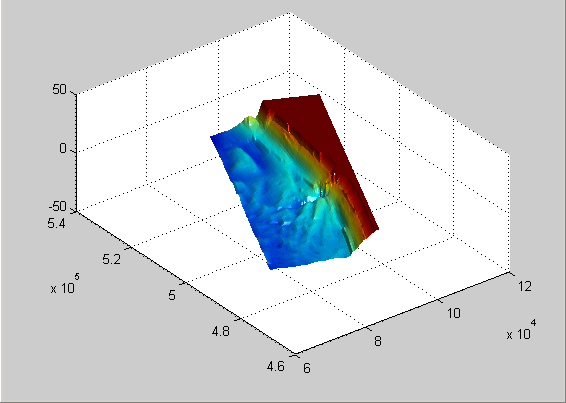
\includegraphics[width=100mm]{matlab/3-3.png}}
\caption{Example of 3D depth plot.}
\label{fig:3-3}
\end{figure}

\section{Read/write grid file: \command{wlgrid}}

\subsection*{Purpose}
Read/write a \DFLOW\ grid file.

\subsection*{Syntax}
\begin{Verbatim}
[X,Y,ENC] = wlgrid('read', FILENAME)
GRID = wlgrid('read', FILENAME)
OK = wlgrid('write', FILENAME, X, Y, ENC)
\end{Verbatim}

\subsection*{Description}
\command{[X, Y, ENC] = wlgrid('read', FILENAME)} reads the grid and enclosure from the Delft3D \file{$\ast$.grd} and \file{$\ast$.enc} files.
X, Y, and enclosure are returned as separate output arguments.
\command{GRID = wlgrid('read', FILENAME)} returns a structure with X, Y, and Enclosure fields.

\command{OK = wlgrid('write', FILENAME, X, Y, ENC)} writes the GRID to \file{$\ast$.grd} and \file{$\ast$.enc} files that can be used by Delft3D.
If the last argument (ENC) is not specified, the enclosure file is not written.

\section{Read/plot velocity field: \command{xyveloc}}

\subsection*{Purpose}
Read velocity data from a \file{trim-*} or \file{com-*} file.

\subsection*{Syntax}
\begin{Verbatim}
[U, V] = xyveloc(NFStruct, TimeStep)
[U, V, W] = xyveloc(NFStruct, Index)
[X, Y, U, V] = xyveloc(NFStruct, TimeStep)
[X, Y, Z, U, V, W] = xyveloc(NFStruct, Index)
[...] = xyveloc(..., 'option')
\end{Verbatim}

\subsection*{Description}
\command{[U, V] = xyveloc(NFStruct, TimeStep)} reads the velocity field at the specified time step from the specified NEFIS file.
By default TimeStep is the last field of the CURTIM or map-series group.
The default NEFIS file is the last opened NEFIS file.

\command{[X, Y, U, V] = xyveloc(NFStruct, TimeStep)} returns not only the velocities, but also the co-ordinates of the grid points at which the velocities are given (water level points).

\command{[U, V, W] = xyveloc(NFStruct, Index)} reads a 3D velocity field (x,y,z components).
\command{[X, Y, Z, U, V, W] = xyveloc(NFStruct, Index)} reads the 3D velocity field (x,y,z components) and returns the 3D co-ordinates of the velocity values.

\command{[...] = XYVELOC(..., 'option')} where the string 'option' equals

\begin{itemize}
\item 'vort': computes the z-component of the vorticity.
Only one output argument is required in this case.
\item 'total', 'fluc', 'mean': reads the total velocity, fluctuation component, or mean velocity field in case of an HLES simulation (trim-file, 2D only).
The default setting is 'total'.
\end{itemize}


\subsection*{Example, \Fref{fig:3-4}}
\begin{Verbatim}
>> vs_use D:\wl\delft3d\tutorial\wave\Siu-Lam\Com-siu
>> [x,y,u,v]=xyveloc;
>> quiver(x,y,u,v)
>> drawgrid('color','g')
>> set(gca,'da',[1 1 1])
>> hold on
>> quiver(x,y,u,v)
\end{Verbatim}

\begin{figure}
\center{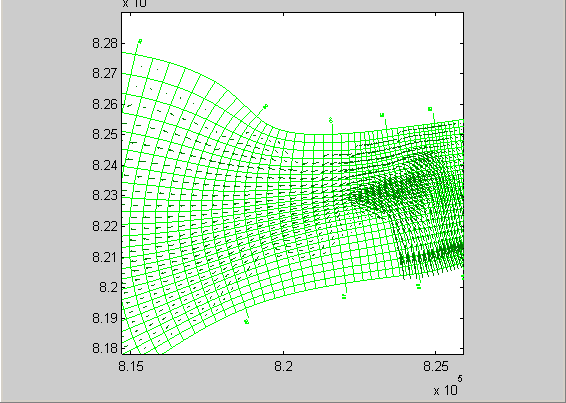
\includegraphics[width=100mm]{matlab/3-4.png}}
\caption{Example of vector velocity plot.}
\label{fig:3-4}
\end{figure}

\section{Generic read data: \command{qpread}}

\subsection*{Purpose}
Get information/data from a data file.
Provides access to the functionality of the QUICKPLOT interface.

\subsection*{Syntax}
\begin{Verbatim}
[DataFields, Dims, NVal] = qpread(FileInfo)
DataProps = qpread(FileInfo)
Size    = qpread(FileInfo, DataProp, 'size')
Size    = qpread(FileInfo, DataFld, 'size')
Times   = qpread(FileInfo, DataProp, 'times')
Times   = qpread(FileInfo, DataFld, 'times')
StNames = qpread(FileInfo, DataProp, 'stations')
StNames = qpread(FileInfo, DataFld, 'stations')
Data    = qpread(FileInfo, DataProp, 'data', t, station, m, n, k)
Data    = qpread(FileInfo, DataFld, 'data', t, station, m, n, k)
Data    = qpread(FileInfo, DataProp, 'griddata', t, station, m, n, k)
Data    = qpread(FileInfo, DataFld, 'griddata', t, station, m, n, k)
\end{Verbatim}

\subsection*{Description}
The \command{qpread} function supports reading data from various data files.
Which data sets can be read from a specific data file can be obtained from the function by one of the following two commands:

\command{[DataFields, Dims, NVal] = qpread(FileInfo)} returns the data fields available from the data file specified using the FileInfo structure.
An acceptable FileInfo can be obtained from any of the following three commands: \command{qpfopen}, \command{qpfile}, \vsuse.
If FileInfo is not specified the last opened NEFIS file is used (same condition applies to the other calls to \command{qpread}).
The variable DataFields is a cell array of strings containing the names of the data sets in the file.
The variable Dims indicates relevant dimensions for the data fields:

\begin{tabular}{ll}
First column of Dims:  & Time step \\
Second column of Dims: & Station name \\
Third column of Dims:  & M \\
Fourth column of Dims: & N \\
Fifth column of Dims:  & K \\
\end{tabular}

NVal equals one for scalar data sets, 2 (or 3) for vector data sets.

\command{DataProps = qpread(FileInfo)} returns a structure containing fields with the above mentioned data and some extra information for internal use by the \command{qpread} and \command{d3d\_qp} functions.

Based on the information returned by either one of these two \command{qpread} statements you may select a data field.
This data field can be identified using its name provided in the DataFields cell array (DataFields{i}) or its record in the DataProps structure (DataProps(i)).
For each data field you can obtain more information by subsequent calls to \command{qpread}.

\begin{Remark}
\item You should not request data for the separator fields with name \command{'-----'}.
\end{Remark}

\command{Size = qpread(FileInfo, DataProp/DataFldName, 'size')} returns a 1 x 5 array containing the maximum size of the five dimensions mentioned above.
The second parameter can be either a string (data field name) or a record from the DataProps structure.
The latter is necessary if the data field name is not unique.

\command{Times = qpread(FileInfo, DataProp/DataFldName, 'times')} returns an array of the times for the specified data field if relevant.

\command{StNames = qpread(FileInfo, DataProp/DataFldName, 'stations')} returns an array of the station names for the specified data field if relevant.

\command{Data = qpread(FileInfo, DataProp/DataFld, 'data', t, station, m, n, k)} returns the data for the specified data field at the indicated time steps, specified station, and M, N, K co-ordinates.
Only those parameters should be specified that have non-zero dimension in Dims and Size.
For a data field at a station often only time and station.
For spatial data sets not the station but a selection of M, N and K.
Following restrictions apply to the retrieval of the data

\begin{itemize}
\item station: index of the station in the StNames array (scalar).
\item 0 (all points) or scalar value (m index).
\item 0 (all points) or scalar value (n index).
\item 0 (all points) or scalar value (k index).
\end{itemize}

\command{Data = qpread(FileInfo, DataProp, 'griddata', t, station, m, n, k)} returns the data and grid for the specified data field at the indicated time steps, specified station, and M, N, K co-ordinates.
In both cases the output argument Data is a structure containing a Time field.
If the data is scalar, the data is returned in the Val field.
If the data is vector data, it is returned as Xcomp and Ycomp fields.

\subsection*{Example, \Fref{fig:3-5}}
\begin{Verbatim}
>> F=qpfopen('D:\wl\delft3d\tutorial\gpp\trim-edw.dat');
>> I=qpread(F);
>> I(9)

ans =

          Name: 'water level'
       DimFlag: [1 0 1 1 0]
    DataInCell: 1
          NVal: 1
       VecType: ''
           Loc: 'z'
        ReqLoc: 'z'
         Loc3D: ''
         Group: 'map-series'
          Val1: 'S1'
          Val2: ''
        SubFld: []
           MNK: 0

>> S=qpread(F,I(9),'griddata')

S =

       X: [87x227 double]
       Y: [87x227 double]
     Val: [87x227 double]
    Time: 7.2942e+005

>> contour(S.X,S.Y,S.Val,50)
>> view(90,90)
>> set(gca,'da',[1 1 100])
\end{Verbatim}

\begin{figure}
\center{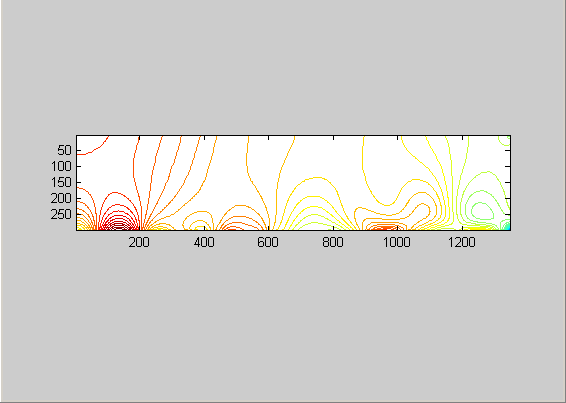
\includegraphics[width=100mm]{matlab/3-5.png}}
\caption{Example of contour plot.}
\label{fig:3-5}
\end{figure}

\section{Generic open file: \command{qpfopen}}

\subsection*{Purpose}
Opening a data file.
Provides access to the functionality of the QUICKPLOT interface.

\subsection*{Syntax}
\begin{Verbatim}
FileInfo=qpfopen('Filename')
FileInfo=qpfopen('DataFile','GridFile')
FileInfo=qpfopen
\end{Verbatim}

\subsection*{Description}
The \command{qpfopen} functions can be used to open all data files that QUICKPLOT can open (see the appendix of the QUICKPLOT manual for an overview of all file formats).

\command{FileInfo=qpfopen('Filename')} opens the specified output file and returns a structure containing data used by the \command{qpread} function.

For WAQ or PART \file{$\ast$.map} files you should also specify an \file{$\ast$.lga} grid file: \command{FileInfo = qpfopen('DataFile', 'GridFile')}
If no grid file is specified then the map file is treated as a history file with an observation point at each location.

\command{FileInfo=qpfopen}
When no arguments are passed to the function, you are asked to specify the file using a standard file selection dialog window.
If you try to open a WAQ or PART \file{$\ast$.map} file, the function asks for the additional grid file.

\section{Get file opened by QUICKPLOT: \command{qpfile}}

\subsection*{Purpose}
Get information about the currently selected file in QUICKPLOT.
Provides access to the functionality of the QUICKPLOT interface.

\subsection*{Syntax}
\begin{Verbatim}
FileInfo=qpfile
\end{Verbatim}

\subsection*{Description}
To make switching between the user interface of QUICKPLOT and MATLAB's command line easier, the \command{qpfile} function provides easy access to the currently selected file in the QUICKPLOT interface.

\command{FileInfo=qpfile} returns the structure of the data file selected in the QUICKPLOT interface.

\svnid{$Id: quickplot.tex 74563 2022-02-13 20:35:17Z jagers $}

\chapter{\DQUICKPLOT\ functionality} \label{Chp:QuickPlot}
The \DQUICKPLOT\ interface can be started by typing \command{d3d\_qp} at the MATLAB command prompt.
This interface is intended to simplify the creation of plots with MATLAB.
Tooltips provide online help for the interface.
The same interface is also available as a standalone program.
This chapter gives only a short introduction; for a detailed description of the interface, you are referred to the \DQUICKPLOT\ manual \citep{QP_UM}.

\begin{figure}
\center{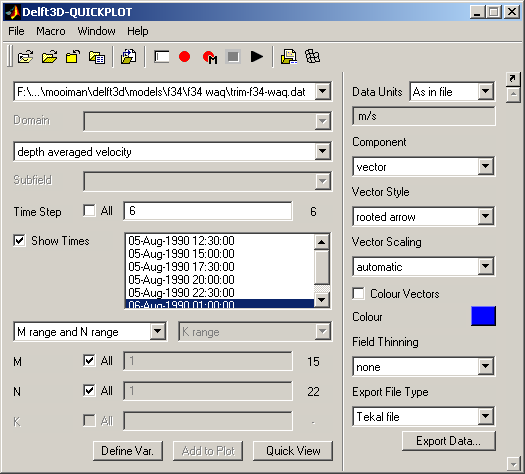
\includegraphics[width=125mm]{matlab/selection_window_qp.png}}
\caption{Selection window of \DQUICKPLOT.}
\label{fig:4.1}
\end{figure}

The interface allows to open NEFIS files and select data fields.
After making a selection of time steps, stations and m, n, k indices, you can either load the data (\button{Load Data} button) or plot the data (by clicking the \button{Quick View} or \button{Quick Animate} button).

The \button{Load Data} button in the lower left corner of the interface is not available in the standalone version, so it is described here.
When the data is loaded using the \button{Load Data} button, a workspace variable called 'data' is created.
If the variable 'data' was already defined any data contained in it will be overwritten without confirmation.
The variable 'data' contains:

\begin{itemize}
\item a field X with the x co-ordinates
\item a field Y with the y co-ordinates
\item a field Z with the z co-ordinates (for 3D data sets only)
\item a field Val with the data is the data is scalar
\item fields XComp, YComp and ZComp when the data is a vector quantity.
\end{itemize}

The same functionality can be accessed from the command line using the command

\begin{Verbatim}
X=d3d_qp('loaddata')
\end{Verbatim}

In this case the data is assigned to the user-specified variable X.
Many of the other functionalities of \DQUICKPLOT\ can also be accessed from the command line.
The general syntax of these commands is:

\begin{Verbatim}
d3d_qp(command_string,...command_parameters...)
\end{Verbatim}

The \command{command\_string} identifies the functionality that should be activated, e.g. 'loaddata', 'openfile' or 'colourbar'.
The \command{command\_parameters} depend on the command chosen, e.g. 'loaddata' does not need any parameter, 'openfile' does not need any parameter either but if a parameter is specified then it should be the name of the file to be opened, and 'colourbar' requires one parameter namely a 1 or 0 to indicate whether a colourbar should be drawn or not.
The details of all these commands is not described here.
The best way to learn these commands is by doing.
Therefore, \DQUICKPLOT\ has several options to display or export the equivalent commands that it is executing when you click on its buttons.
These display options can be accessed from the Macro menu of \DQUICKPLOT\ as shown in \Fref{fig:4.2}.

\begin{figure}
\center{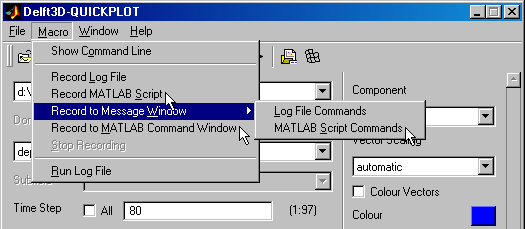
\includegraphics[width=100mm]{matlab/4-2.png}}
\caption{Display/export options for QUICKPLOT\ commands.}
\label{fig:4.2}
\end{figure}

For exporting/displaying the MATLAB commands associated with the various functionalities of \DQUICKPLOT, the following three options are available:

\begin{itemize}
\item Record MATLAB Script.
Records the commands directly to a MATLAB .m file.
\item Record to Message Window, MATLAB Script Commands.
Records the commands in a separate window of \DQUICKPLOT.
The commands cannot be copied from this window, but the recorded commands can be saved to a text file.
\item Record to MATLAB Command Window (not available in the standalone version of \DQUICKPLOT).
Echoes the commands to the MATLAB Command Window from which they can be easily copied.
When using MATLAB's diary option, the echoed commands will also end up in the diary file.
\end{itemize}

Both \DQUICKPLOT\ log files and MATLAB script files containing \DQUICKPLOT\ calls can be run using the Run Log File menu item of \DQUICKPLOT.
The MATLAB script files may also contain other single line MATLAB function calls (not supported in standalone mode).
Scripts containing multi-line MATLAB constructs cannot be run from within the \DQUICKPLOT\ interface.

When the data is plotted or animated a new figure is opened.
Scaling of axes, vector length and colours is automatic.
This implies that during an animation colour scaling, vector length scaling and plot extent may vary.
The plot extent and colour scaling can be set using the MATLAB commands \command{axis}, \command{set}, \command{gca} and \command{colorbar}.
For example:

\begin{Verbatim}
axis([xmin xmax ymin ymax]) % set the axes extent
\end{Verbatim}

and

\begin{Verbatim}
set(gca,'clim',[cmin cmax]) % set the colour limits
colorbar % update the colourbar
\end{Verbatim}

\begin{figure}
\center{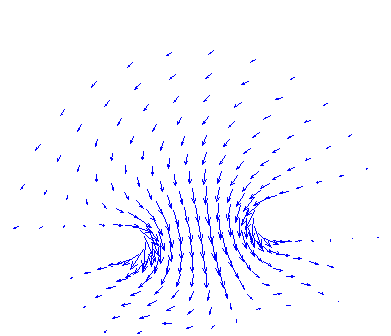
\includegraphics{matlab/standard_vector_plot.png}}
\caption{Example of \DQUICKPLOT\ figure.}
\label{fig:4.3}
\end{figure}

In case of an animation, plotting can be stopped by either closing the figure or selecting the Stop option from the Animation menu in the figure of the plot.
When the data set contains multiple time steps, a scroll bar will be plotted in the lower left corner of the plot figure.
You can use this to change the time step of the plot.

\begin{Remark}
\item The figure files saved by the standalone version of \DQUICKPLOT\ are compatible with MATLAB 6.5.
It does not support files created with newer MATLAB versions.
\item Access to netCDF files and data on OPeNDAP enabled websites requires the 'mexnc' and 'snctools' toolboxes available from \url{http://mexcdf.sourceforge.net/}.
The files of those toolboxes are now included in the netcdf subdirectory of the \DMATLAB distribution and should be automatically added to the search path when running \command{d3d\_qp} or \command{qpfopen}.
\end{Remark}

\svnid{$Id: references.tex 74563 2022-02-13 20:35:17Z jagers $}

\nonumchapter{References} \label{chp:references}

\bibliography{../common/deltares_manual}


\cleardoublepage
%
\newpage
\pagestyle{empty}
\mbox{}
\includepdf[pages=2,offset=-72 -70]{pictures/delft3d-cover_matlab.pdf} % links-rechts past precies
\end{document}
